\documentclass[aspectratio=43]{beamer}

\usetheme{Boadilla}
\setbeamertemplate{footline}[page number]{}
\setbeamertemplate{navigation symbols}{}

\usepackage{times}
\usepackage{tikz}
\usefonttheme{structurebold}
\usepackage{listings}
\usepackage{hyperref}

\definecolor{commgreen}{rgb}{0,0.6,0}
% Suppress the navigation bar
\beamertemplatenavigationsymbolsempty

\newenvironment{changemargin}[1]{% 
  \begin{list}{}{% 
    \setlength{\topsep}{0pt}% 
    \setlength{\leftmargin}{#1}% 
    \setlength{\rightmargin}{1em}
    \setlength{\listparindent}{\parindent}% 
    \setlength{\itemindent}{\parindent}% 
    \setlength{\parsep}{\parskip}% 
  }% 
  \item[]}{\end{list}} 

\title{Tutorial 02---Implement Scalable Servers with Non-blocking / Asynchronous I/O}
\subtitle{ECE 459: Programming for Performance}
\author{David Xi Cheng \\ \href{mailto:david.cheng@uwaterloo.ca}{david.cheng@uwaterloo.ca}}
\institute{University of Waterloo}
\date{January 21, 2015}

\begin{document}

%%%%%%%%%%%%%%%%%%%%%%%%%%%%%%%%%%%%%%%%%%%%%%%%%%%%%%%%%%%%%%%%%%%%%%%%%%%%%%%%
\begin{frame}[plain]
  \titlepage
\end{frame}

%%%%%%%%%%%%%%%%%%%%%%%%%%%%%%%%%%%%%%%%%%%%%%%%%%%%%%%%%%%%%%%%%%%%%%%%%%%%%%%%
\begin{frame}
  \frametitle{References}

  \begin{itemize}
  	\item \href{http://beej.us/guide/bgnet/}{Beej's Guide to Network Programming}
  	\item \href{http://www.kegel.com/c10k.html}{The C10K problem}
	\item \href{https://cs.uwaterloo.ca/~brecht/papers/getpaper.php?file=ols-2004.pdf}{L. Gammo, T. Brecht, A. Shukla and D. Pariag. Comparing and Evaluating epoll, select and poll Event Mechanisms. In Proceedings of the Ottawa Linux Symposium, 2004}
	\item \href{https://www.usenix.org/legacy/events/hotos03/tech/full_papers/vonbehren/vonbehren.pdf}{v. Behren, J. Robert, J. Condit, and E. A. Brewer. Why Events Are a Bad Idea (for High-Concurrency Servers). In HotOS, 2003.}
	\item \href{http://www.eecs.harvard.edu/~mdw/papers/seda-sosp01.pdf}{M. Welsh, D. Culler, and E. Brewer. SEDA: An Architecture for Well-Conditioned, Scalable Internet Services. In SOSP, 2001.}
  \end{itemize}
  \end{frame}
%%%%%%%%%%%%%%%%%%%%%%%%%%%%%%%%%%%%%%%%%%%%%%%%%%%%%%%%%%%%%%%%%%%%%%%%%%%%%%%%

\part{How to Write a Server}
\begin{frame}
\partpage
\end{frame}
%%%%%%%%%%%%%%%%%%%%%%%%%%%%%%%%%%%%%%%%%%%%%%%%%%%%%%%%%%%%%%%%%%%%%%%%%%%%%%%%
\begin{frame}[fragile]
  \frametitle{How to Write a Server?}
  \begin{enumerate}
  	\item create, bind, listen 
  \end{enumerate}
  
  \begin{lstlisting}[language=C,basicstyle=\ttfamily\footnotesize,commentstyle=\color{commgreen},keywordstyle=\color{blue}]
  //create a socket file descriptor
  int socket( int domain, int type, int protocol );
 
  //bind socket to a particular address:port pair
  int bind( int sockfd, struct sockaddr *addr, int addrlen );
  
  //listen for incoming connections
  int listen( int sockfd, int backlog );
  \end{lstlisting}
\end{frame}
%%%%%%%%%%%%%%%%%%%%%%%%%%%%%%%%%%%%%%%%%%%%%%%%%%%%%%%%%%%%%%%%%%%%%%%%%%%%%%%%

%%%%%%%%%%%%%%%%%%%%%%%%%%%%%%%%%%%%%%%%%%%%%%%%%%%%%%%%%%%%%%%%%%%%%%%%%%%%%%%%
\begin{frame}[fragile]
  \frametitle{Create, Bind, Listen Example\\ (Init and Create)}

  \begin{lstlisting}[language=C++,basicstyle=\ttfamily\footnotesize,commentstyle=\color{commgreen},keywordstyle=\color{blue},breaklines=true]
  int create_bind_listen( int port ){
      struct sockaddr_in server_addr;
  
      //init server addr struct
      memset( &server_addr, 0, sizeof(server_addr) );
      server_addr.sin_family = AF_INET;
      server_addr.sin_port = htons( port );
      server_addr.sin_addr.s_addr = htonl( INADDR_ANY );
      
      //create
      int server_sock = socket(AF_INET, SOCK_STREAM, 0);
      if( server_sock < 0 ){
          return -1;
      }
      ...
  \end{lstlisting}
\end{frame}
%%%%%%%%%%%%%%%%%%%%%%%%%%%%%%%%%%%%%%%%%%%%%%%%%%%%%%%%%%%%%%%%%%%%%%%%%%%%%%%%

%%%%%%%%%%%%%%%%%%%%%%%%%%%%%%%%%%%%%%%%%%%%%%%%%%%%%%%%%%%%%%%%%%%%%%%%%%%%%%%%
\begin{frame}[fragile]
  \frametitle{Create, Bind, Listen Example\\ (Bind and Listen)}

  \begin{lstlisting}[language=C++,basicstyle=\ttfamily\footnotesize,commentstyle=\color{commgreen},keywordstyle=\color{blue},breaklines=true]
	    //bind
	    int ret = bind( server_sock, (struct sockaddr *) &server_addr, sizeof(server_addr) );

	    if( ret < 0 ){
	        close( server_sock );
	        return -1;
	    }

	    //listen
	    ret = listen( server_sock, 5 );
	    if( ret < 0 ){
	        close( server_sock );
	        return -1;
	    }
	    
	    return server_sock;
	}
  \end{lstlisting}
\end{frame}
%%%%%%%%%%%%%%%%%%%%%%%%%%%%%%%%%%%%%%%%%%%%%%%%%%%%%%%%%%%%%%%%%%%%%%%%%%%%%%%%

%%%%%%%%%%%%%%%%%%%%%%%%%%%%%%%%%%%%%%%%%%%%%%%%%%%%%%%%%%%%%%%%%%%%%%%%%%%%%%%%
\begin{frame}[fragile]
  \frametitle{How to Write a Server}

   \begin{enumerate}
   \setcounter{enumi}{1}
   \item accept a connection
    \end{enumerate}
    \begin{lstlisting}[language=C++,basicstyle=\ttfamily\footnotesize,commentstyle=\color{commgreen},keywordstyle=\color{blue},breaklines=true]
   //accept a connection
   int accept( int socked, struct sockaddr *addr, socklen_t *addrlen );
   \end{lstlisting}
   
   \begin{enumerate}
   \setcounter{enumi}{2}
   \item communicate with a client
   \end{enumerate}
   
   \begin{lstlisting}[language=C++,basicstyle=\ttfamily\footnotesize,commentstyle=\color{commgreen},keywordstyle=\color{blue},breaklines=true]
   //receive messages
   int recv( int sockfd, void *buf, int len, int flags );
   
   //send messages
   int send( int sockfd, const void *msg, int len, int flags );
   \end{lstlisting}
\end{frame}
%%%%%%%%%%%%%%%%%%%%%%%%%%%%%%%%%%%%%%%%%%%%%%%%%%%%%%%%%%%%%%%%%%%%%%%%%%%%%%%%

%%%%%%%%%%%%%%%%%%%%%%%%%%%%%%%%%%%%%%%%%%%%%%%%%%%%%%%%%%%%%%%%%%%%%%%%%%%%%%%%
\begin{frame}[fragile]
  \frametitle{Trivial Server (Synchronous)}

\begin{lstlisting}[language=C++,basicstyle=\ttfamily\footnotesize,commentstyle=\color{commgreen},keywordstyle=\color{blue},breaklines=true]
int main(){
    int server_sock;
    if( (server_sock = create_bind_listen(PORT_NUMBER)) < 0 ){
        exit( EXIT_FAILURE );
    }
    
    struct sockaddr_in client_addr;
    socklen_t client_addr_len = sizeof( client_addr );
    int client_fd;
    
    while( true ){
        client_fd = accept( server_sock, (struct socked *) &client_addr, &client_addr_len );
        if( client_fd < 0 ) {    exit( EXIT_FAILURE );    }
        
        //communications happen here
        
        close( client_fd );
    }
}
   \end{lstlisting}
\end{frame}
%%%%%%%%%%%%%%%%%%%%%%%%%%%%%%%%%%%%%%%%%%%%%%%%%%%%%%%%%%%%%%%%%%%%%%%%%%%%%%%%

%%%%%%%%%%%%%%%%%%%%%%%%%%%%%%%%%%%%%%%%%%%%%%%%%%%%%%%%%%%%%%%%%%%%%%%%%%%%%%%%
\begin{frame}
  \frametitle{Synchronous Server}

\hspace*{2em} \begin{minipage}{.8\textwidth}
Serve one client at a time.\\[2em]

It doesn't work in the presence of,
\begin{itemize}
\item concurrent connections
\begin{itemize}\item connections would timeout if not accepted in time\end{itemize}
\item persistent connections
\begin{itemize}\item could serve only one client \end{itemize}
\end{itemize}

\vspace{2em}
\begin{center}
{\LARGE Not Scalable!}
\end{center}
\end{minipage}
\end{frame}
%%%%%%%%%%%%%%%%%%%%%%%%%%%%%%%%%%%%%%%%%%%%%%%%%%%%%%%%%%%%%%%%%%%%%%%%%%%%%%%%
\part{How to Write a Scalable Server}

\begin{frame}
 \partpage
\end{frame}
%%%%%%%%%%%%%%%%%%%%%%%%%%%%%%%%%%%%%%%%%%%%%%%%%%%%%%%%%%%%%%%%%%%%%%%%%%%%%%%%
\begin{frame}
  \frametitle{How to Write a Scalable Server}
\hspace*{2em} \begin{minipage}{.8\textwidth}
What are the options
\begin{itemize}
\item Serve one client with each server thread
\begin{itemize}
\item multi-thread/process model
\end{itemize}
\vspace{0.5em}
\item Serve many clients with each server thread
\begin{itemize}
\item non-blocking Multiplexing\\
{\footnotesize \tt select, poll, epoll(Linux), kqueue(BSD)} \\[0.5em]
\item asynchronous I/O\\
{\footnotesize \tt callback upon completion}
\end{itemize}
\end{itemize}
\end{minipage}
\end{frame}
%%%%%%%%%%%%%%%%%%%%%%%%%%%%%%%%%%%%%%%%%%%%%%%%%%%%%%%%%%%%%%%%%%%%%%%%%%%%%%%%
\begin{frame}[fragile]
  \frametitle{Multi-Thread/Process Model}
  Each server thread/process serves only one client\\
  \begin{itemize}
  \item simpler programming style
  \item handles concurrent connections
  \item performance degradation after too many threads/processes\\
  {\scriptsize (due to memory and context-switch overhead)}\\
  {\tiny (although, people would argue to do better with user-level scheduling)}
  \end{itemize}
  
  \begin{center}
   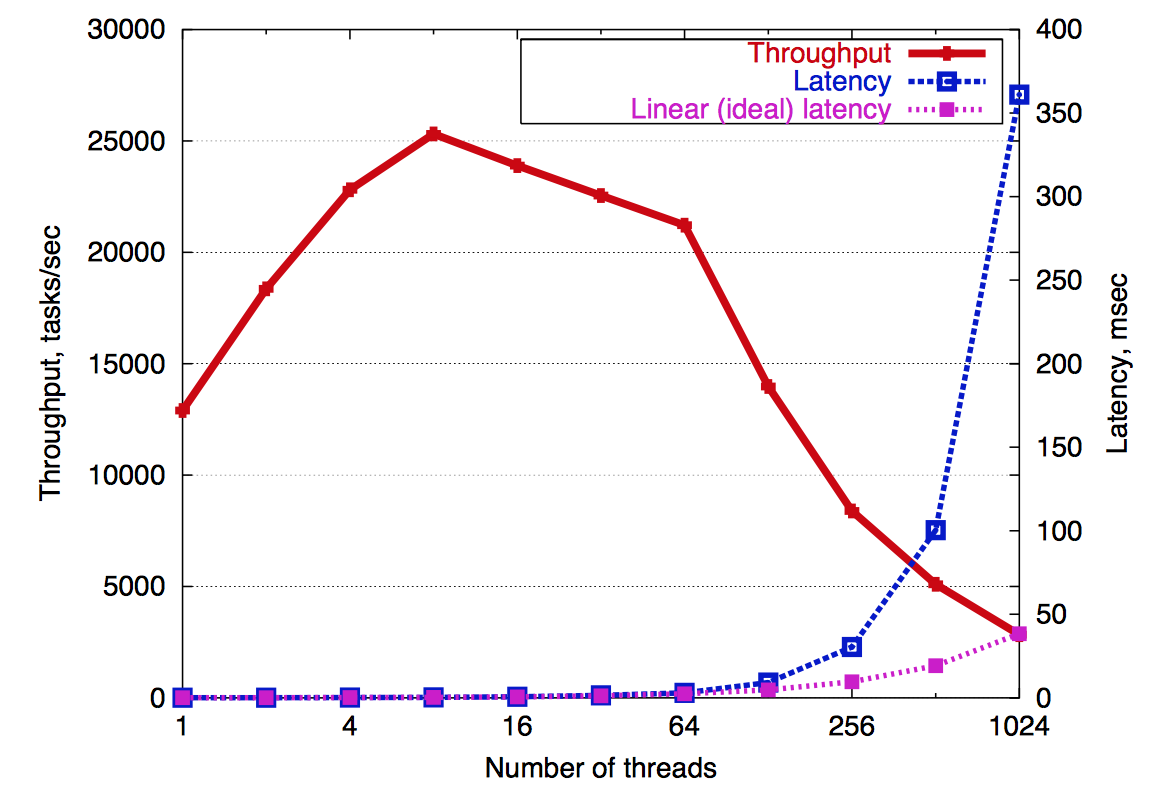
\includegraphics[scale=0.3]{server_mp_degrade.png}\\
   {\tiny Threaded server performance degradation on 4wy 500MHz Pentium III with 2 GB memory\footnote{\tiny Figure 2, SEDA: An Architecture for Well-Conditioned Scalable Internet Services, SOSP 2001}}
  \end{center}
\end{frame}
%%%%%%%%%%%%%%%%%%%%%%%%%%%%%%%%%%%%%%%%%%%%%%%%%%%%%%%%%%%%%%%%%%%%%%%%%%%%%%%%
\begin{frame}[fragile]
  \frametitle{Multi-Thread/Process Model Example}
  \begin{lstlisting}[language=C++,basicstyle=\ttfamily\footnotesize,commentstyle=\color{commgreen},keywordstyle=\color{blue},breaklines=true]

int main(){
    int server_sock;
    if( (server_sock = create_bind_listen(PORT_NUMBER)) < 0 ){
        exit( EXIT_FAILURE );
    }
    
    struct sockaddr_in client_addr;
    socklen_t client_addr_len = sizeof( client_addr );
    int client_fd;
    
    while( true ){
        client_fd = accept( server_sock, (struct socked *) &client_addr, &client_addr_len );
        if( client_fd < 0 ) {    exit( EXIT_FAILURE );    }
        
        //create a separate thread/process to
        //communicate with the client
    }
}
\end{lstlisting}
\end{frame}
%%%%%%%%%%%%%%%%%%%%%%%%%%%%%%%%%%%%%%%%%%%%%%%%%%%%%%%%%%%%%%%%%%%%%%%%%%%%%%%%


%%%%%%%%%%%%%%%%%%%%%%%%%%%%%%%%%%%%%%%%%%%%%%%%%%%%%%%%%%%%%%%%%%%%%%%%%%%%%%%%
\begin{frame}[fragile]
  \frametitle{Non-blocking Multiplexing}
  Each server thread/process serves multiple clients.\\
  \begin{itemize}
  \item Multiplexed with notification facilities, i.e., select, poll and epoll.
  \end{itemize}
  Generalized Event Loop
  \begin{enumerate}
  \item create/modify set(s) of file descriptors that require readiness notifications.
  \item wait on select/poll/epoll until one or more fds become ready.
  \item select/poll/epoll returns with hints of which fds are ready to read/write or have exceptions.
  \item handle those fds appropriately.
  \item repeat from step 1.
  \end{enumerate}
  \vspace{1em}
  \begin{center}
  {\large Use non-blocking I/O to avoid blocking the event loop!}
  \end{center}
\end{frame}
%%%%%%%%%%%%%%%%%%%%%%%%%%%%%%%%%%%%%%%%%%%%%%%%%%%%%%%%%%%%%%%%%%%%%%%%%%%%%%%%

%%%%%%%%%%%%%%%%%%%%%%%%%%%%%%%%%%%%%%%%%%%%%%%%%%%%%%%%%%%%%%%%%%%%%%%%%%%%%%%%
\begin{frame}
  \frametitle{Blocking v.s. Non-blocking I/O}

\hspace*{2em} \begin{minipage}{.8\textwidth}
In previous examples,\\[1em]
all of {\tt accept,send,recv} operations would block the entire thread if,
\begin{itemize}
\item no clients to {\tt accept}.
\item no data to {\tt recv}.
\item {\tt send} buffer is full.
\end{itemize}
\vspace{1em}
\end{minipage}
\end{frame}
%%%%%%%%%%%%%%%%%%%%%%%%%%%%%%%%%%%%%%%%%%%%%%%%%%%%%%%%%%%%%%%%%%%%%%%%%%%%%%%%

%%%%%%%%%%%%%%%%%%%%%%%%%%%%%%%%%%%%%%%%%%%%%%%%%%%%%%%%%%%%%%%%%%%%%%%%%%%%%%%%
\begin{frame}[fragile]
  \frametitle{Blocking v.s. Non-blocking I/O}

\hspace*{2em} \begin{minipage}{.8\textwidth}
To avoid blocking the thread in the above conditions, we need to use non-blocking I/O instead.\\[1em]
In the non-blocking mode, -1 is immediately returned with {\tt errno} set to {\tt EWOULDBLOCK}, if the operation would block.\\[1em]
To set a file descriptor as non-blocking, we need to 
  \begin{lstlisting}[language=C++,basicstyle=\ttfamily\footnotesize,commentstyle=\color{commgreen},keywordstyle=\color{blue},breaklines=true]
  //retrieve original flags of the FD
  int flags = fcntl( fd, F_GETFL, 0 );
  
  //add an O_NONBLOCK flag
  flags |= O_NONBLOCK
  
  //reset the flag of the FD
  fcntl( fd, F_SETFL, flags );
  \end{lstlisting}

\end{minipage}
\end{frame}
%%%%%%%%%%%%%%%%%%%%%%%%%%%%%%%%%%%%%%%%%%%%%%%%%%%%%%%%%%%%%%%%%%%%%%%%%%%%%%%%

%%%%%%%%%%%%%%%%%%%%%%%%%%%%%%%%%%%%%%%%%%%%%%%%%%%%%%%%%%%%%%%%%%%%%%%%%%%%%%%%
\begin{frame}[fragile]
  \frametitle{Select}
  \hspace*{2em} \begin{minipage}{.8\textwidth}
  \begin{lstlisting}[language=C++,basicstyle=\ttfamily\footnotesize,commentstyle=\color{commgreen},keywordstyle=\color{blue},breaklines=true]
	int select( int nfds, fd_set *readfds, fd_set *writefds, fd_set *exceptfds, struct timeval *timeout );
   \end{lstlisting}
   \end{minipage}
   \begin{itemize}
	 \item first introduced in 4.2 BSD Unix in 1983.
	 \item takes three {\tt fd\_set} to monitor read/write/except readiness.
	 \item blocks until one or more file descriptors become ready.
	 \item {\tt fd\_set} is essentially a bitmap, fixed in size of {\tt FD\_SETSIZE}, 1024 by default. (i.e., support at most 1024 file descriptors)
	 \item the {\tt fd\_set} bitmaps are overridden upon return, need to be restored before each call.
	 \end{itemize}
    \vspace{1em} 
     \hspace*{2em}\begin{minipage}{.8\textwidth}
   You may access {\tt fd\_set} with the following macros.
   \end{minipage}
     \begin{lstlisting}[language=C++,basicstyle=\ttfamily\footnotesize,commentstyle=\color{commgreen},keywordstyle=\color{blue},breaklines=true]
     void FD_CLR( int fd, fd_set *set );
     int  FD_ISSET( int fd, fd_set *set );
     void FD_SET( int fd, fd_set *set );
     void FD_ZERO( fd_set *set );
   \end{lstlisting}
\end{frame}
%%%%%%%%%%%%%%%%%%%%%%%%%%%%%%%%%%%%%%%%%%%%%%%%%%%%%%%%%%%%%%%%%%%%%%%%%%%%%%%%

%%%%%%%%%%%%%%%%%%%%%%%%%%%%%%%%%%%%%%%%%%%%%%%%%%%%%%%%%%%%%%%%%%%%%%%%%%%%%%%%
\begin{frame}[fragile]
  \frametitle{Select Example (init fd\_set)}
       \begin{lstlisting}[language=C++,basicstyle=\ttfamily\footnotesize,commentstyle=\color{commgreen},keywordstyle=\color{blue},breaklines=true]
int main() {
    /* create, bind, listen first */
    
    int fd_max;
    fd_set sock_fds, read_fds;
    
    FD_ZERO( &sock_fds ); FD_ZERO( &read_fds );
    //add server_sock to the fd set
    FD_SET( server_sock, &sock_fds );
    //server_sock is the largest fd as of now
    fd_max = server_sock;
    ...
    \end{lstlisting}
\end{frame}
%%%%%%%%%%%%%%%%%%%%%%%%%%%%%%%%%%%%%%%%%%%%%%%%%%%%%%%%%%%%%%%%%%%%%%%%%%%%%%%%


%%%%%%%%%%%%%%%%%%%%%%%%%%%%%%%%%%%%%%%%%%%%%%%%%%%%%%%%%%%%%%%%%%%%%%%%%%%%%%%%
\begin{frame}[fragile]
  \frametitle{Select Example (event loop) }
 \begin{lstlisting}[language=C++,basicstyle=\ttfamily\tiny,commentstyle=\color{commgreen},keywordstyle=\color{blue},breaklines=true]
    while( true ){
        //make a copy of sock_fds
        read_fds = sock_fds;
        
        if( select(fd_max+1, &read_fds, NULL, NULL, NULL) == -1 ){
            /* handles select error here */
        }
        
        //read_fds is now overridden with hints of fd readiness.
        for( int i = 0; i <= fd_max; ++i ) {
            if( FD_ISSET(i, &read_fds) ){
                //fd i is now ready
                if( i == server_sock ){ //server_sock is ready to accept
                    /* accept a client here */
                    
                    //add client_sock to fd_set
                    FD_SET( client_sock, &sock_fds );
                    //reset fd_max
                    if( client_sock > fd_max ){ fd_max = client_sock; }
                }
                
                else{ //client_sock is ready to read
                    /* communicate with the client */
                
                    if( /* done with the client */ ) {
                        FD_CLR( i, &sock_fds ); 
                        close( i );
                    }
                }
            } //if
        } //for
    } //while
} //main
       \end{lstlisting}
\end{frame}
%%%%%%%%%%%%%%%%%%%%%%%%%%%%%%%%%%%%%%%%%%%%%%%%%%%%%%%%%%%%%%%%%%%%%%%%%%%%%%%%

%%%%%%%%%%%%%%%%%%%%%%%%%%%%%%%%%%%%%%%%%%%%%%%%%%%%%%%%%%%%%%%%%%%%%%%%%%%%%%%%
\begin{frame}[fragile]
  \frametitle{Poll}
  \begin{lstlisting}[language=C++,basicstyle=\ttfamily\footnotesize,commentstyle=\color{commgreen},keywordstyle=\color{blue},breaklines=true]
int poll( struct pollfd *fds, nfds_t nfds, int timeout );   
\end{lstlisting}
   \begin{itemize}
	 \item introduced to Linux since kernel version 2.1.23 in 1997
	 \item takes an array of {\tt struct pollfd} to monitor fd readiness\\{\scriptsize (as opposed to bitmaps in {\tt select})}.
	 \begin{lstlisting}[language=C++,basicstyle=\ttfamily\scriptsize,commentstyle=\color{commgreen},keywordstyle=\color{blue},breaklines=true]
struct pollfd {
    int   fd;         /* file descriptor */
    short events;     /* requested events */
    short revents;    /* returned events */
};
\end{lstlisting}
	 {\scriptsize (fd number, monitored/occurred events are encapsulated as different fields) }
	 \item blocks until one or more file descriptors become ready.
	 \item only changes {\tt pollfd.revents} upon return.\\ {\scriptsize (do not need to recover fd set before each call)}
	 \item no upper limit for array size.
   \end{itemize}
\end{frame}
%%%%%%%%%%%%%%%%%%%%%%%%%%%%%%%%%%%%%%%%%%%%%%%%%%%%%%%%%%%%%%%%%%%%%%%%%%%%%%%%

%%%%%%%%%%%%%%%%%%%%%%%%%%%%%%%%%%%%%%%%%%%%%%%%%%%%%%%%%%%%%%%%%%%%%%%%%%%%%%%%
\begin{frame}[fragile]
  \frametitle{Poll Example}
\begin{lstlisting}[language=C++,basicstyle=\ttfamily\footnotesize,commentstyle=\color{commgreen},keywordstyle=\color{blue},breaklines=true]
int main(){
    /* create, bind, listen first */
    
    //use vector for pollfd array
    std::vector<struct pollfd> sock_fds;

    //create the first pollfd for server_sock
    struct pollfd pfd;
    server_pfd.fd = server_sock;
    server_pfd.events = POLLIN;
    
    sock_fds.push_back( pfd );

    \end{lstlisting}
\end{frame}
%%%%%%%%%%%%%%%%%%%%%%%%%%%%%%%%%%%%%%%%%%%%%%%%%%%%%%%%%%%%%%%%%%%%%%%%%%%%%%%%

%%%%%%%%%%%%%%%%%%%%%%%%%%%%%%%%%%%%%%%%%%%%%%%%%%%%%%%%%%%%%%%%%%%%%%%%%%%%%%%%
\begin{frame}[fragile]
  \frametitle{Poll Example (event loop)}
\begin{lstlisting}[language=C++,basicstyle=\ttfamily\tiny,commentstyle=\color{commgreen},keywordstyle=\color{blue},breaklines=true]
    while( true ){  
        if( poll(&sock_fds[0], sock_fds.size(), -1 ) < 0) {
            /* handle poll error here */
        }
    
        //iterate through sock_fds for readiness
        for( auto it = sock_fds.begin(); it != sock_fds.end(); ++it ) {            
            if( !((*it).revents & POLLIN) ){ continue; }

            if( (*it).fd == server_sock ){ //server_sock is ready to accept
                    /* accept a client here */
                    
                    //add client_sock to sock_fds
                    pfd.fd = client_sock; pfd.events = POLLIN;
                    sock_fds.push_back( pfd );
                }       
            }

            else{ //client_sock is ready to read
                /* communicate with the client here */
                
                if( /* done with the client */ ) { //remove the client from poll queue
                    close( (*it).fd );
                    sock_fds.erase( it );
                    --it;
                }
            } //else
        } //for
    } //while
} //main

\end{lstlisting}
\end{frame}
%%%%%%%%%%%%%%%%%%%%%%%%%%%%%%%%%%%%%%%%%%%%%%%%%%%%%%%%%%%%%%%%%%%%%%%%%%%%%%%%

%%%%%%%%%%%%%%%%%%%%%%%%%%%%%%%%%%%%%%%%%%%%%%%%%%%%%%%%%%%%%%%%%%%%%%%%%%%%%%%%
\begin{frame}[fragile]
  \frametitle{select, poll v.s. epoll}
     Both select and poll need to scan the entire fd set per call.\\
     Time Complexity: linear to the number of connections.\\
     \begin{center}
     \large generally doesn't scale beyond 10,000 connections!
     \end{center}
     
     epoll, event-driven notification facility
     \begin{itemize}
     \item new interface introduced since Linux kernel 2.5.44 in 2002.
     \item tracks the state changes of file descriptors, without iterating through the entire fd set.
     \item Time Complexity: linear to number of \emph{active} connections.
     \end{itemize}
\end{frame}
%%%%%%%%%%%%%%%%%%%%%%%%%%%%%%%%%%%%%%%%%%%%%%%%%%%%%%%%%%%%%%%%%%%%%%%%%%%%%%%%

%%%%%%%%%%%%%%%%%%%%%%%%%%%%%%%%%%%%%%%%%%%%%%%%%%%%%%%%%%%%%%%%%%%%%%%%%%%%%%%%
\begin{frame}[fragile]
  \frametitle{select, poll v.s. epoll}
  \begin{center}
  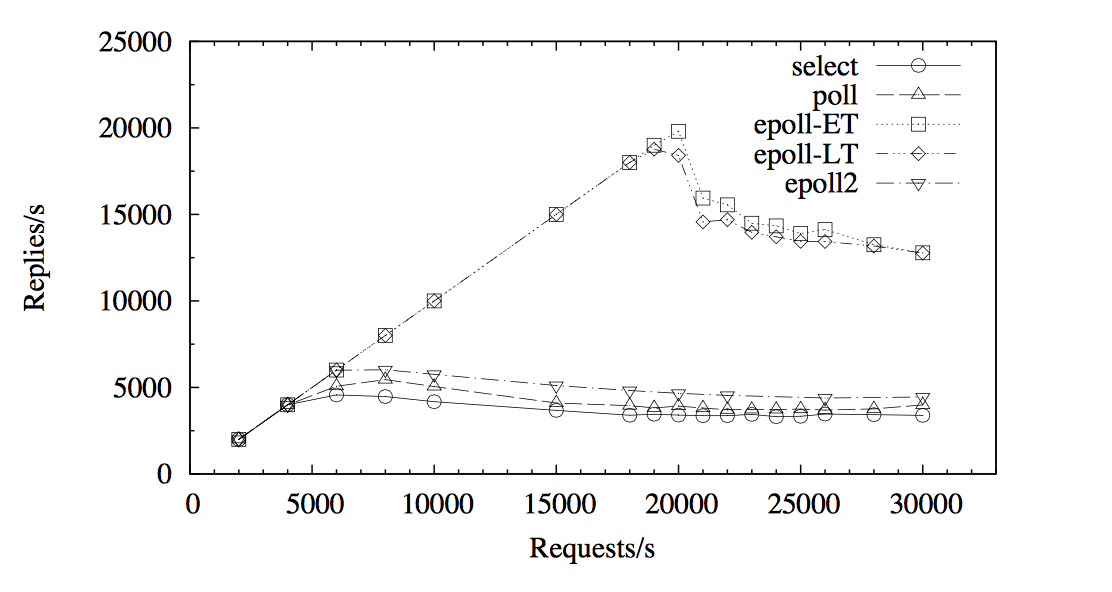
\includegraphics[scale=0.5]{select_poll_epoll_perf.png}\\
  {\footnotesize $\mu$server performance comparison with different notification facilities.\footnote{\tiny Figure 5, Comparing and Evaluating epoll, select, and poll Event Mechanisms, Linux Symposium Vol.01, 2004}}
  \end{center}
\end{frame}
%%%%%%%%%%%%%%%%%%%%%%%%%%%%%%%%%%%%%%%%%%%%%%%%%%%%%%%%%%%%%%%%%%%%%%%%%%%%%%%%

%%%%%%%%%%%%%%%%%%%%%%%%%%%%%%%%%%%%%%%%%%%%%%%%%%%%%%%%%%%%%%%%%%%%%%%%%%%%%%%%
\begin{frame}[fragile]
  \frametitle{Epoll}
    \begin{lstlisting}[language=C++,basicstyle=\ttfamily\scriptsize,commentstyle=\color{commgreen},keywordstyle=\color{blue},breaklines=true]
//deprecated as of kernel version 2.6.8
//the size argument is since ignored,
//in favour of dynamic queue size.
int epoll_create( int size );

//the flags argument could be of,
//0, same as epoll_create() behaviour.
//EPOLL_CLOEXEC, with close-on-exec flag set.
int epoll_create1( int flags );

//op:EPOLL_CTL_ADD to register a new fd
//op:EPOLL_CTL_MOD to change an existing fd
//op:EPOLL_CTL_DEL to delete an existing fd
int epoll_ctl( int epfd, int op, int fd, struct epoll_event *event );

//epoll_event.events is a bit set for monitored events
//epoll_event.data.fd stores the file descriptor to monitor
struct epoll_event {
    uint32_t     events;      /* Epoll events */
    epoll_data_t data;        /* User data variable */
};

\end{lstlisting}
\end{frame}
%%%%%%%%%%%%%%%%%%%%%%%%%%%%%%%%%%%%%%%%%%%%%%%%%%%%%%%%%%%%%%%%%%%%%%%%%%%%%%%%

%%%%%%%%%%%%%%%%%%%%%%%%%%%%%%%%%%%%%%%%%%%%%%%%%%%%%%%%%%%%%%%%%%%%%%%%%%%%%%%%
\begin{frame}[fragile]
  \frametitle{Epoll}
    \begin{lstlisting}[language=C++,basicstyle=\ttfamily\footnotesize,commentstyle=\color{commgreen},keywordstyle=\color{blue},breaklines=true]
int epoll_wait( int epfd, struct poll_event *events, int maxevents, int timeout );
\end{lstlisting}

\begin{itemize}
\item {\tt epfd} is the epoll file descriptor that you want to use.
\item active FDs will be copied to the {\tt events} array upon return.
\item {\tt maxevents} is the max num of active events per call.
\item blocks until one or more FDs are ready.
\end{itemize}
\end{frame}
%%%%%%%%%%%%%%%%%%%%%%%%%%%%%%%%%%%%%%%%%%%%%%%%%%%%%%%%%%%%%%%%%%%%%%%%%%%%%%%%

%%%%%%%%%%%%%%%%%%%%%%%%%%%%%%%%%%%%%%%%%%%%%%%%%%%%%%%%%%%%%%%%%%%%%%%%%%%%%%%%
\begin{frame}[fragile]
  \frametitle{Epoll Example}
\begin{lstlisting}[language=C++,basicstyle=\ttfamily\footnotesize,commentstyle=\color{commgreen},keywordstyle=\color{blue},breaklines=true]
int main(){
    /* create, bind, listen here */
    
    int epfd = epoll_create1( 0 );
    if( epfd < 0 ){
        /* handle epoll error here */
    }

    //adding server_sock to the epoll queue
    struct epoll_event ev, events[EPOLL_QUEUE_LEN];
    ev.events = EPOLLIN;
    ev.data.fd = server_sock;
    if( epoll_ctl(epfd, EPOLL_CTL_ADD, server_sock, &ev) < 0 ){
        /* handle epoll_ctl error here */
    }
    ...
   \end{lstlisting}
\end{frame}
%%%%%%%%%%%%%%%%%%%%%%%%%%%%%%%%%%%%%%%%%%%%%%%%%%%%%%%%%%%%%%%%%%%%%%%%%%%%%%%%

%%%%%%%%%%%%%%%%%%%%%%%%%%%%%%%%%%%%%%%%%%%%%%%%%%%%%%%%%%%%%%%%%%%%%%%%%%%%%%%%
\begin{frame}[fragile]
  \frametitle{Epoll Example (event loop)}
\begin{lstlisting}[language=C++,basicstyle=\ttfamily\tiny,commentstyle=\color{commgreen},keywordstyle=\color{blue},breaklines=true]
    while( true ){  
        num_fds = epoll_wait( epfd, events, EPOLL_QUEUE_LEN, -1 );

        if( num_fds < 0 ){
            /* handle epoll_wait error here */
        }
    
        //FDs in events are active
        for( int i = 0; i < num_fds; ++i ) {
            if( events[i].data.fd == server_sock ){ //server_sock is ready to accept
                
                /* accept a client here */
                
                // you may reuse the ev struct
                ev.events = EPOLLIN;
                ev.data.fd = client_sock;
                if( epoll_ctl(epfd, EPOLL_CTL_ADD, client_sock, &ev) < 0 ){
                    /* handle epoll_ctl error here */
                } 
            }

            else{ //client_sock is ready to read
                
                /* communicate with the client here */
                
                if( /* done with the client */ ){ //remove the client from epoll queue               
                    if( epoll_ctl( epfd, EPOLL_CTL_DEL, events[i].data.fd, NULL ) < 0 ){
                        /* handle epoll_ctl error here */
                    }
                    
                    close( events[i].data.fd );
                } //if
            }  //else
        }  //for
    }  //while
} //main
   \end{lstlisting}
\end{frame}
%%%%%%%%%%%%%%%%%%%%%%%%%%%%%%%%%%%%%%%%%%%%%%%%%%%%%%%%%%%%%%%%%%%%%%%%%%%%%%%%

%%%%%%%%%%%%%%%%%%%%%%%%%%%%%%%%%%%%%%%%%%%%%%%%%%%%%%%%%%%%%%%%%%%%%%%%%%%%%%%%
\begin{frame}[fragile]
  \frametitle{Edge v.s. Level-Triggered}
   We mentioned that epoll tracks state changes of FDs,\\
   epoll could work under two modes,\\
   \begin{itemize}
   \item Edge-Triggered {\scriptsize notify only when an FD changes from not ready to ready}\\
   {\footnotesize e.g., won't notify again if you don't empty the buffer first }
   \item Level-Triggered {\scriptsize notify whenever an FD is ready}\\
   {\footnotesize e.g., will always notify if there is data in the buffer }
   \end{itemize}
   
   epoll works under LT mode by default,\\this is how you could change it to ET,
   \begin{lstlisting}[language=C++,basicstyle=\ttfamily\footnotesize,commentstyle=\color{commgreen},keywordstyle=\color{blue},breaklines=true]
    struct epoll_event ev;
    ev.events = EPOLLIN | EPOLLET;
    ev.data.fd = sockfd;
    if( epoll_ctl(epfd, EPOLL_CTL_ADD, sockfd, &ev) < 0 ){
        /* handle epoll_ctl error here */
    }
   \end{lstlisting}
   
   
\end{frame}
%%%%%%%%%%%%%%%%%%%%%%%%%%%%%%%%%%%%%%%%%%%%%%%%%%%%%%%%%%%%%%%%%%%%%%%%%%%%%%%%

\end{document}
